\section{Hardware for real-world experiments}
    \subsection{Robots}
        This section will present the robots we will use in real-world experiments. We will use two robotic platforms: Husky and Spot.\\\\
        \bfc{Husky}\\
        Husky is a medium all-terrain robot developed by Clearpath Robotics. It is a four-wheeled robot with a payload capacity of 75 kg. The weight of this robot without the payload is 50 kg, and its maximal speed is $1\:\mathrm{[m/s]}$. This robot is mainly used outside of urban areas. The photo of Husky is shown in figure \ref{fig:husky}.\\
        More information is available at the Clearpath Robotics website\footnote{\url{https://clearpathrobotics.com/husky-unmanned-ground-vehicle-robot/}}.\\\\
        \bfc{Spot}\\
        The spot is a medium all-terrain robot developed by Boston Dynamics. It is a four-legged robot with a payload capacity of 14 kg. The weight of this robot without the payload is 33 kg, and its maximal speed is $1.6\:\mathrm{[m/s]}$. This robot is mainly used in urban areas. The photo of the spot is shown in figure \ref{fig:spot}.\\
        More information is available at the Boston Dynamics website\footnote{\url{https://www.bostondynamics.com/sites/default/files/inline-files/spot-specifications.pdf}}.\\

        \begin{figure}[H]
            \centering
            \begin{subfigure}[b]{0.49\textwidth}
                \centering
                \includegraphics[width=\textwidth]{images/husky.jpg}
                \caption{Robot Husky.}
                \label{fig:husky}
            \end{subfigure}
            \begin{subfigure}[b]{0.49\textwidth}
                \centering
                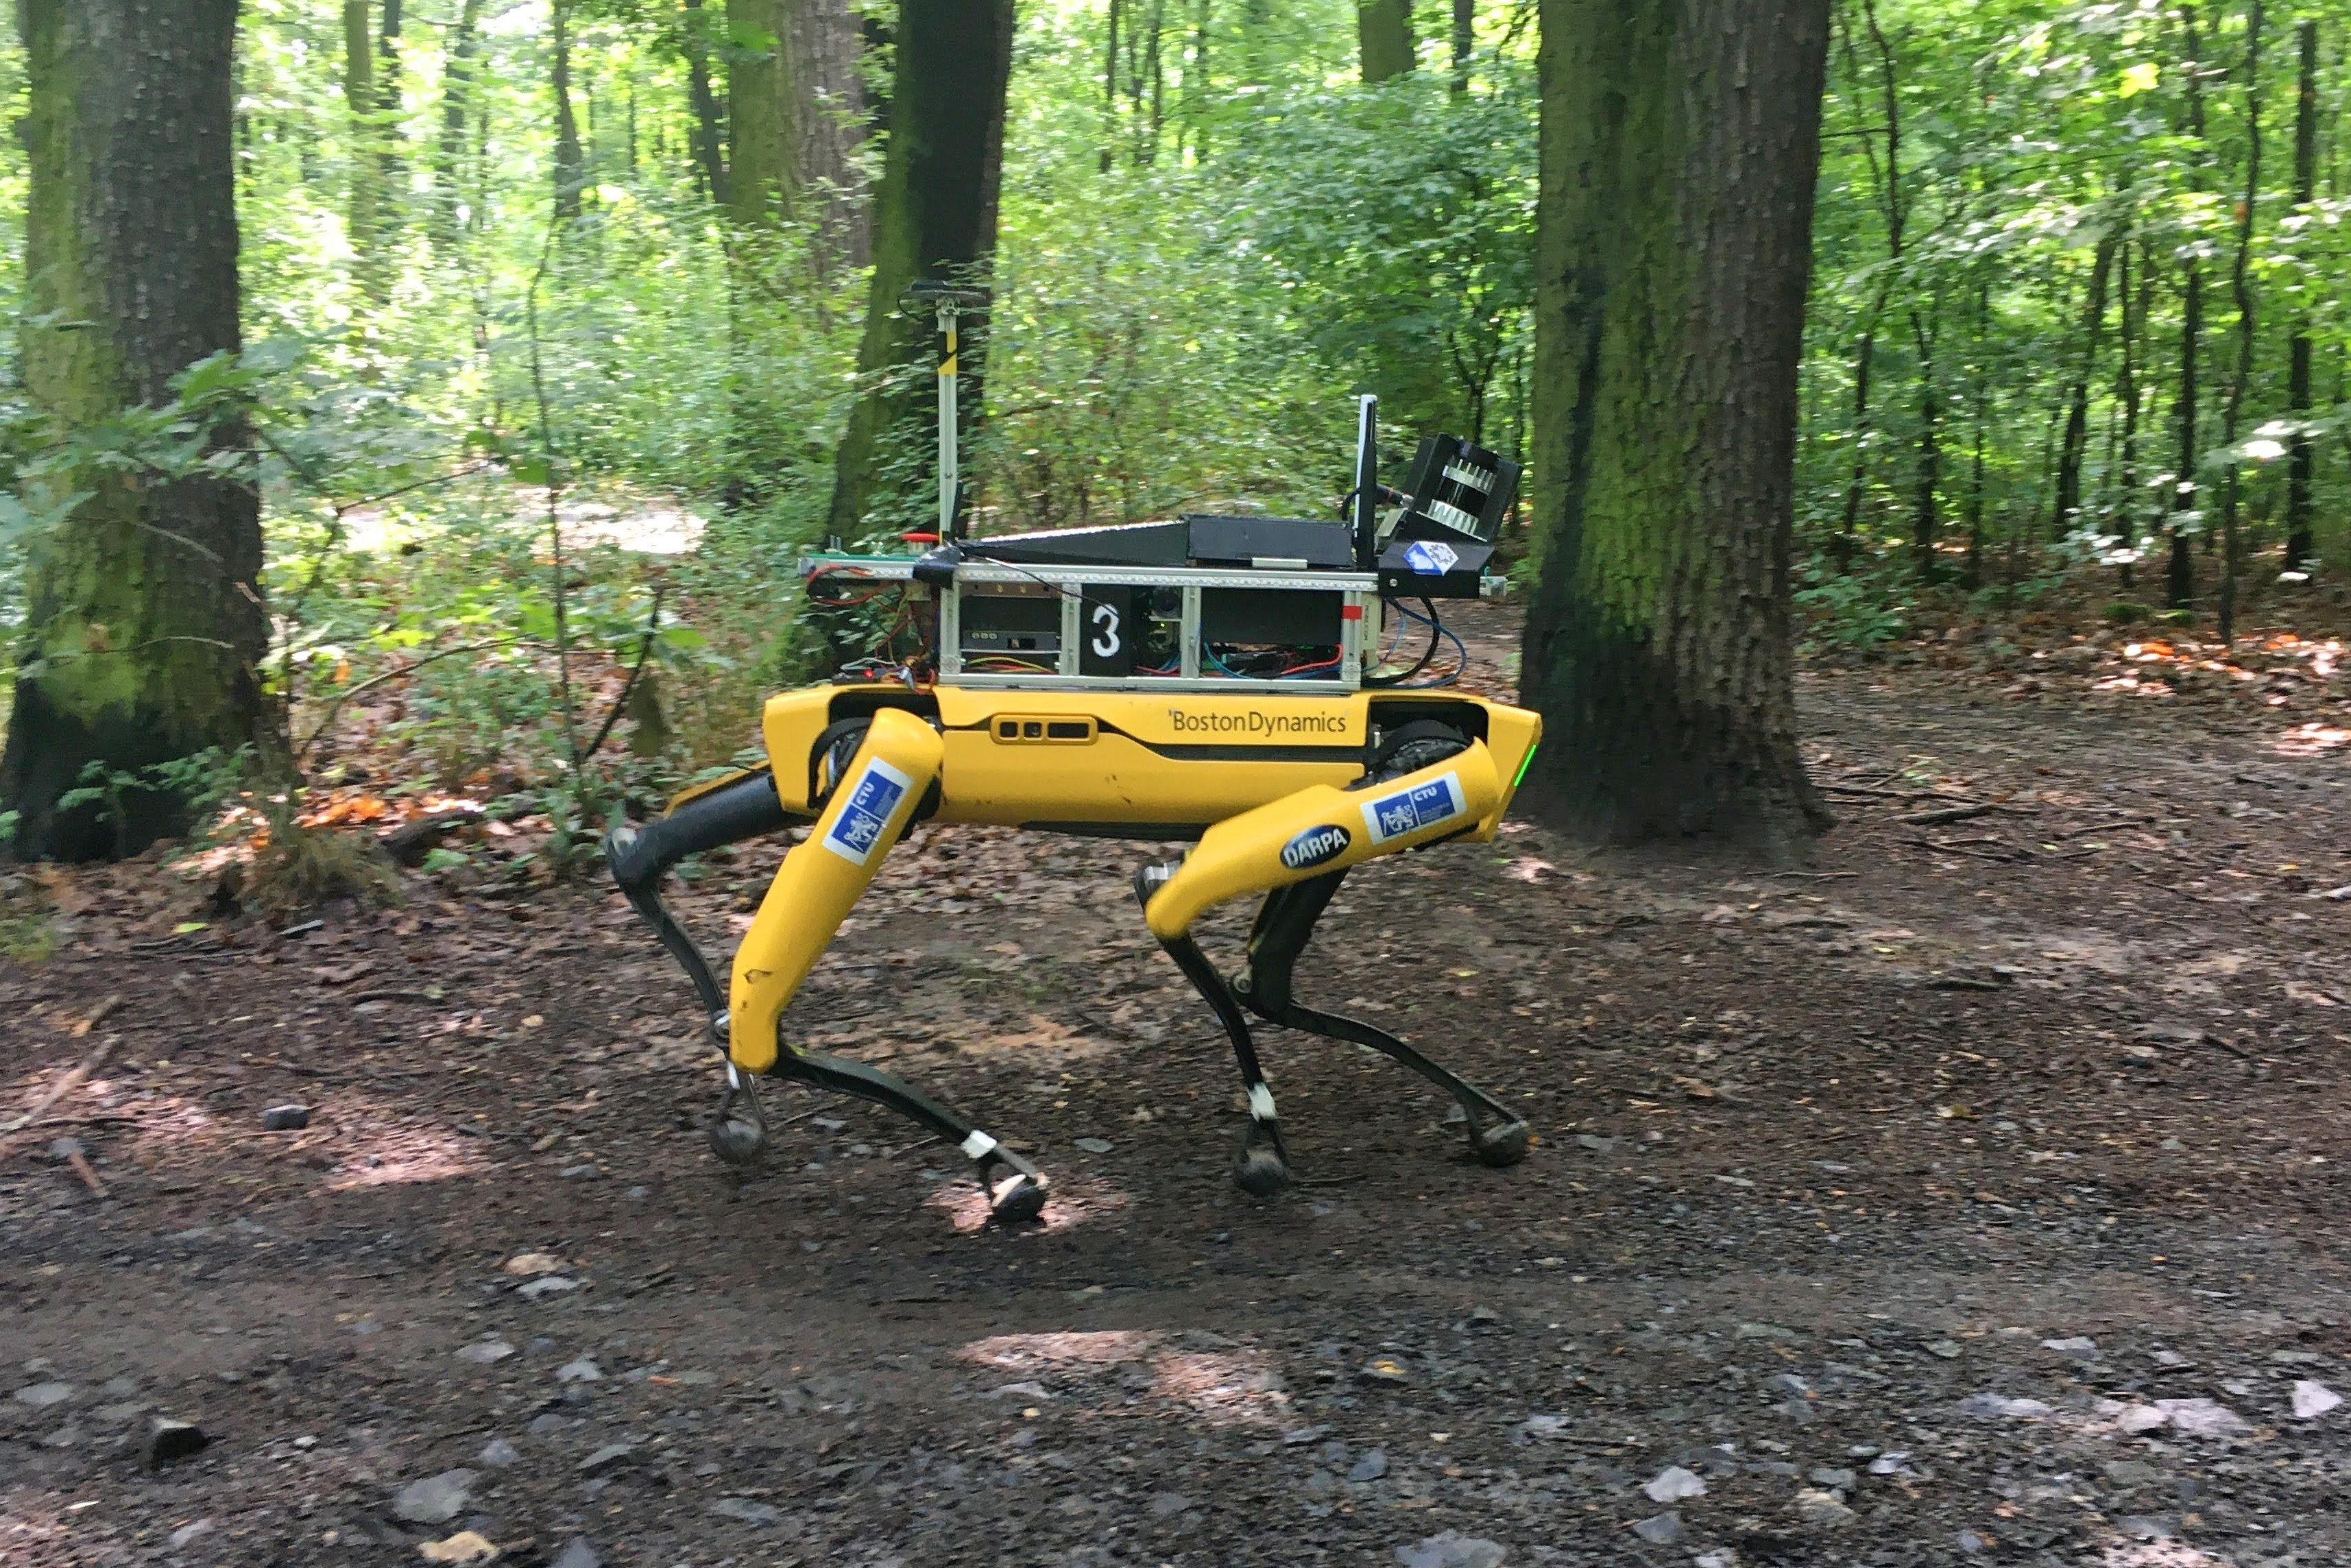
\includegraphics[width=\textwidth]{images/spot3.jpg}
                \caption{Robot Spot.}
                \label{fig:spot}
            \end{subfigure}
            \caption{Robots used in the real-world experiments.}
        \end{figure}
        \noindent Photos are courtesy of CRAS at FEE CTU.

    \subsection{Sensors}
        The robots we use are highly dependent on the sensors we attach to them. Without them, the possibilities and options for the mission are limited. We will use some sensors directly and some indirectly. The indirect usage of sensors is due to the need to work with detected vehicles and other obstacles. This detection is not in the scope of our work but is instrumental to its success.\\\\
        \bfc{Magnetometer}\\
            This is a sensor we use directly. We use it to determine the heading of our robot and help it position itself perpendicular to the road it will try to cross.\\\\
        \bfc{Camera}\\
            Our robots are fitted with cameras pointing forward, backwards, left, right, and up. This sensor is mostly used to determine the classification of obstacles rather than detecting the obstacles themselves.\\
            The cameras on our robots are GigE Basler ace2 PRO.\\\\
        \bfc{LiDAR}\\
            Another sensor our robots are equipped with is LiDAR (laser imaging, detection, and ranging). This sensor detects incoming vehicles and determines their speed and position vectors. It is probably the most important sensor due to its processed data being our algorithm's main switching condition.\\
            The LiDARs used on our robots are Ouster OS0-128.\\\\
        \bfc{GPS}\\
            Robots also have a GPS sensor. We use this sensor for precise localization of the robots in global coordinates.\\
                    The GPS sensors we use are Emlid Reach M+.